\documentclass{article}
\usepackage{amsmath}
\usepackage[utf8]{inputenc}
\usepackage{listings}
\usepackage{graphicx}

\graphicspath{ {../results/} }

\lstset{
	basicstyle=\footnotesize,
	numbers=left,
	tabsize=3,
	title=\lstname,
	breaklines=true
}

\addtolength{\oddsidemargin}{-.875in}
\addtolength{\evensidemargin}{-.875in}
\addtolength{\textwidth}{1.75in}

\addtolength{\topmargin}{-.875in}
\addtolength{\textheight}{1.75in}

\title{Lernverfahren autonomer Roboter - Übung 10}
\author{G10\\ Andre Osse\\ Waldemar Stockmann\\ Markus Strehling\\ Tobias Hahn}	
	
\begin{document}
\maketitle
\newpage
\section{Multilayer Neural Network and Backpropagation}

\subsection{Implementation}
Das Netzwerk wurde wie gewünscht implementiert, der Code ist wie folgt:

\lstinputlisting{../code/multi.py}

\paragraph{}
Außerdem wurde der Test ausgeführt, mit folgendem Ergebnis:
\begin{lstlisting}
Fully connected layer (20 nodes, 20 x 11 weights)
Fully connected layer (10 nodes, 10 x 21 weights)
Fully connected layer (3 nodes, 3 x 11 weights)
Checking gradients up to 5 positions after decimal point...OK
\end{lstlisting}

\subsection{Sinus lernen}
Der Sinus wurde gelernt, folgende Ausgaben wurden mit dem Testprogramm erzielt:
\paragraph{}
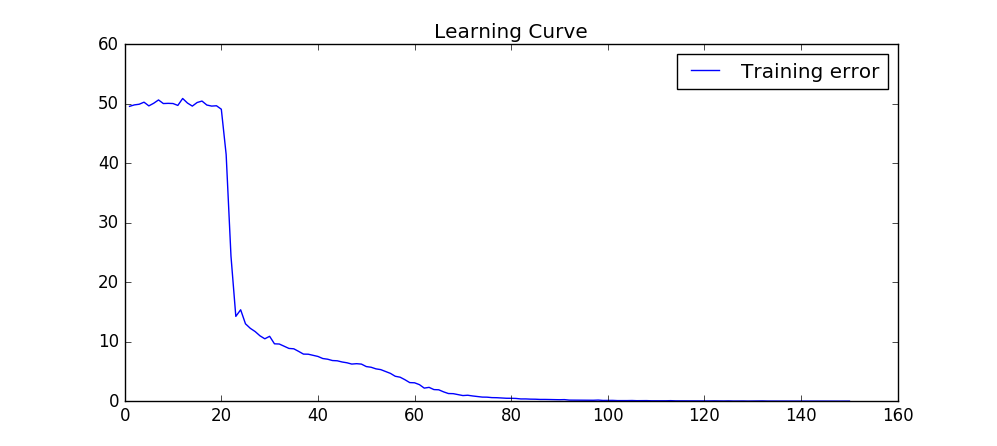
\includegraphics[width=\textwidth]{learning_rate.png}
\paragraph{}
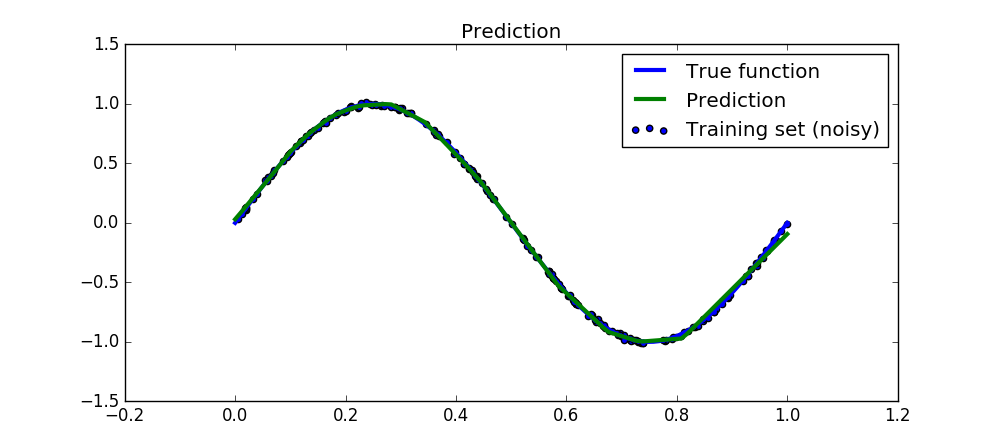
\includegraphics[width=\textwidth]{prediction.png}

\section{Roboter lernen}
\subsection{Code}
\lstinputlisting{../code/sac.py}

\subsection{Output}
\begin{lstlisting}
## Linear Regression ##
Train data
Dimension 1: nMSE = 7.36 %
Dimension 2: nMSE = 10.26 %
Dimension 3: nMSE = 9.11 %
Dimension 4: nMSE = 5.12 %
Dimension 5: nMSE = 14.56 %
Dimension 6: nMSE = 27.44 %
Dimension 7: nMSE = 6.52 %
Test data
Dimension 1: nMSE = 7.42 %
Dimension 2: nMSE = 10.10 %
Dimension 3: nMSE = 9.18 %
Dimension 4: nMSE = 5.13 %
Dimension 5: nMSE = 14.13 %
Dimension 6: nMSE = 28.24 %
Dimension 7: nMSE = 6.46 %
## Neural Net ##
Train data
Dimension 1: nMSE = 5.96 %
Dimension 2: nMSE = 4.94 %
Dimension 3: nMSE = 4.13 %
Dimension 4: nMSE = 2.23 %
Dimension 5: nMSE = 6.49 %
Dimension 6: nMSE = 7.95 %
Dimension 7: nMSE = 2.82 %
Test data
Dimension 1: nMSE = 5.93 %
Dimension 2: nMSE = 4.88 %
Dimension 3: nMSE = 4.20 %
Dimension 4: nMSE = 2.22 %
Dimension 5: nMSE = 6.26 %
Dimension 6: nMSE = 8.02 %
Dimension 7: nMSE = 2.95 %
\end{lstlisting}
\end{document}
